\section{Mining Ontology-Annotated Data Using Hypergraphs}
\label{sec:method}
Besides the common graph-theoretic model of RDF as labeled, directed multi-graphs, Hayes has established that RDF can be also represented as hypergraphs (bipartite graphs)~\cite{GraphModelRDF}. This result constitutes an important aspect of the theoretical basis of this paper and is discussed in detail below.

\subsection{Hypergraph Representation for Ontologies and RDF Data}
The RDF graph is defined as a set of RDF triples and can be visualized as a \emph{directed labeled graph} as follows:
\begin{center}\ovalbox{subject} $\stackbin[]{predicate}{\xrightarrow{\hspace*{2cm}}}$ \ovalbox{object}\;.\end{center}

RDF makes the artificial distinction between resources and properties, which leads to incongruous graph representations. Consider the following example:

\begin{figure}[tbh]
\begin{center}
\begin{tabular}{c}
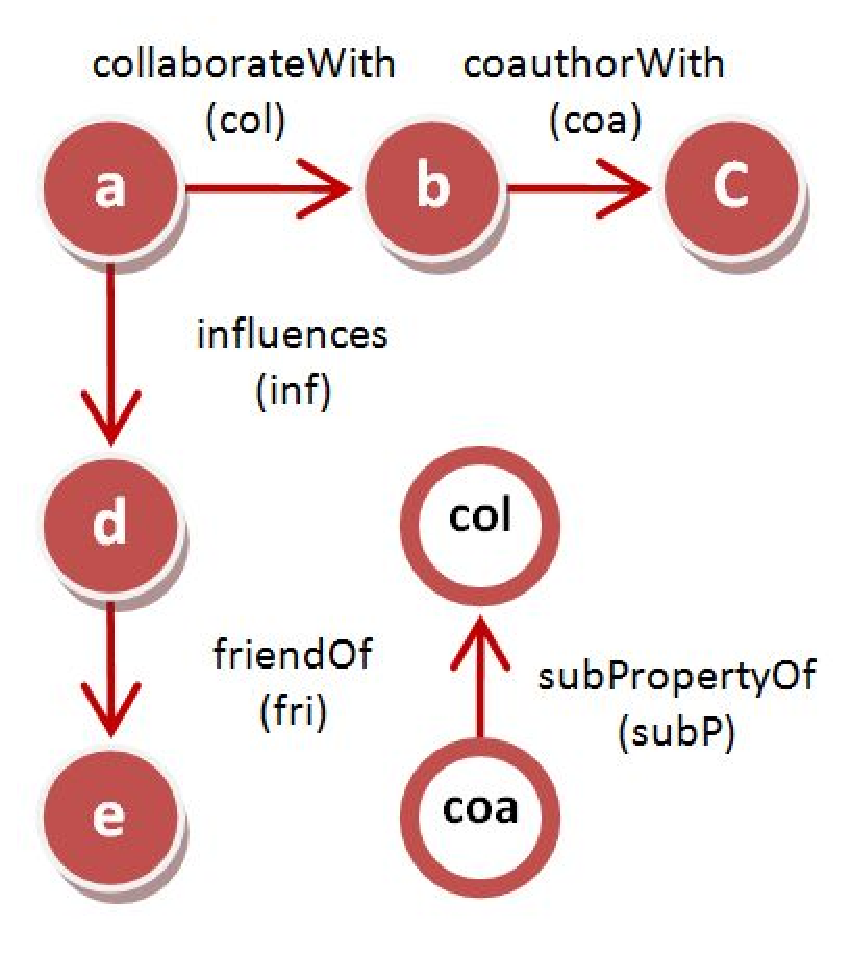
\includegraphics[width=.22\textwidth]{fig/reg_graph.eps}\\
(A)\\
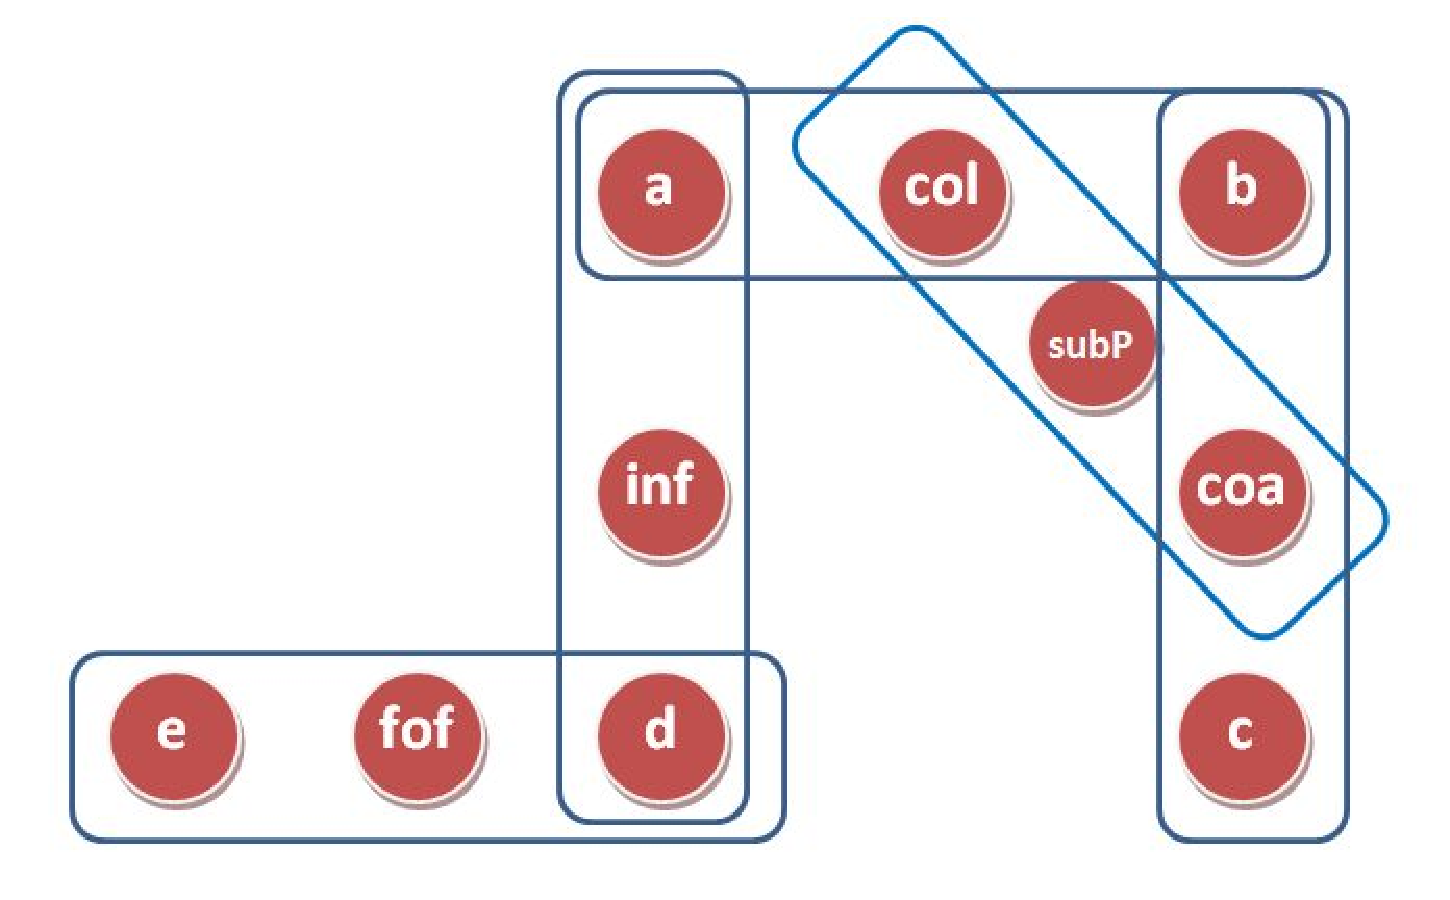
\includegraphics[width=.35\textwidth]{fig/hypergraph.eps}\\
(B)\\
\end{tabular}
\end{center}
\caption{\label{fig:graphcomp} As a directed graph representation (A) the nodes and edges for \emph{col} and \emph{coa} are incongruously intermixed, where the hypergraph (B) seamlessly avoids the discrepancy.}
\end{figure}

\begin{myexp}
\label{graphcomp}
\emph{(\textbf{Discrepancy of the RDF directed labeled graph})}
A set of RDF statements describes the following relationships among people: $\langle a$ $collaborateWith$ $b\rangle$, $\langle b$ $coauthorWith$ $c\rangle$, $\langle a$ $influences$ $d\rangle$ and $\langle d$ $friendOf$ $e\rangle$; where $a$, $b$, $c$, $d$, and $e$ are variables representing people. Futhermore, $\langle coauthorWith $ $subProperty$ $collaborationWith\rangle$. In this case, the graph representation mixes nodes and edges incongruously. See Figure~\ref{fig:graphcomp}.
\end{myexp}

As illustrated in Figure~\ref{fig:graphcomp}, a hypergraph representation of the RDF statements avoids such discrepancies.  A \emph{hypergraph}~\cite{Hypergraph} is a generalization of a traditional graph where edges, called hyperedges, can connect more than two vertices. If each edge in a hypergraph covers the same number of nodes, it's called an $r$-uniform hypergraph, $r$ being the number of nodes on each edge. Any RDF Graph can be represented by a simple, ordered, 3-uniform hypergraph, in which an RDF triple corresponds to a hypergraph edge, the nodes being the subject, predicate and object in this order~\cite{GraphModelRDF}. In this way, ontological statements can be represented in a coherent graph model (Fig.~\ref{fig:graphcomp}(B)).

\begin{mydef}
\emph{(\textbf{Hypergraph})}
Formally, a hypergraph $G = (V,E)$, is a pair in which $V$ is the vertex set and $E$ is the hyperedge set where each $e \in E$ is a subset of $V$. A weighted hypergraph is a hypergraph that has a positive number $w(e)$ associated with each hyperedge $e$; called the weight of hyperedge $e$: Denote a weighted hypergraph by $G = (V,E,w)$.
%The degree of a vertex $v \in V$, $d(v)$, is defined as $d(v) = \sum_{v\in V, e\in E}{w(e)}$.
%The degree of a hyperedge $e$, denoted as $\delta(e)$, is the number of vertices in $e$, i.e. $\delta(e)=|e|$. A hyperedge $e$ is said to be incident with a vertex $v$ when $v \in e$. The hypergraph incidence matrix $\mathbf{H} \in \mathbb{R}^{|V| \times |E|}$ is defined as
%\begin{equation}
%\notag h(v,e)=\left\{\begin{array}{cl}
%	   1, & v \in e \\
%	   0, & otherwise
%	   \end{array}\right.
%\end{equation}
%Throughout the rest of the paper, the diagonal matrix forms for $\delta(e)$, $w(e)$, $d(v)$ are denoted as $\mathbf{D}_e$, $\mathbf{W} \in \mathbb{R}^{|E|}$, and $\mathbf{D}_v \in \mathbb{Z}^{|V|}$, respectively.
\end{mydef}

Furthermore, A hypergraph $HG = (V, E)$ can be transformed to a \emph{bipartite graph} $BG$ as follows:
%\begin{mydef}
%\emph{(\textbf{Transformation from RDF hypergraph (HG) to RDF bipartite graph (BG)})}
the node sets $V$ and $E$ be the two parts of $BG$, and $(v_1, e_1)$ is connected with an edge if and only if vertex $v_1$ is contained in the hyperedge $e_1$ in $HG$. In other words, the incidence matrix of $HG$ can be viewed as the node adjacency (biadjacency) matrix of the bipartite graph. The proof that $BG$ is indeed bipartite is straightforward and we omit it for lack of space.

%\end{mydef}
%\begin{figure}[tbh]
%\centering
%\begin{minipage}[c]{0.58\textwidth}\centering
%\[ \bordermatrix{ ~       &  \text{~a~}  &  \text{~b~}  &  \text{~c~}  &  \text{~d~}  &  \text{~e~}  &   \text{coa} &   \text{col} &   \text{inf} &   \text{fof} &   \text{subP}\cr
%                  E_1~~   &   1   &   1   &       &       &       &       &   1   &       &       &       \cr
%                  E_2~~   &       &   1   &   1   &       &       &   1   &       &       &       &       \cr
%                  E_3~~   &   1   &       &       &   1   &       &       &       &   1   &       &       \cr
%                  E_4~~   &       &       &       &   1   &   1   &       &       &       &   1   &       \cr
%                  E_5~~   &       &       &       &       &       &   1   &   1   &       &       &    1}
%\]
%\end{minipage}
%\hfill
%\begin{minipage}[c]{0.38\textwidth}\centering
%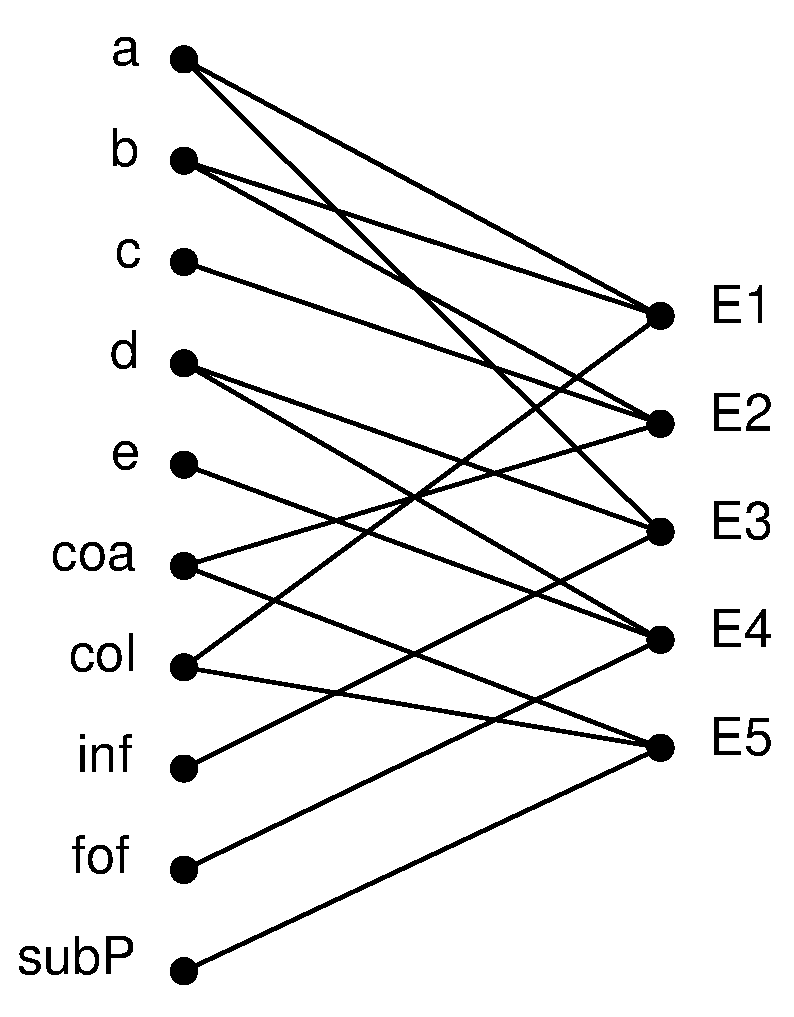
\includegraphics[width=.7\textwidth]{fig/BG-black.eps}
%\end{minipage}
%\caption{\label{fig:incidence}Incidence matrix representing the hypergraph of figure~\ref{fig:graphcomp}(B) and the corresponding incidence graph.}
%\end{figure}

Bipartite graphs are well-known from their efficient computational properties and we demonstrate next that the RDF bipartite graph can be efficiently mined for \emph{semantically associated itemsets}.

%
%\begin{myexp}[\textbf{Hypergraph incidence matrix and corresponding bipartite graph}]
%\label{incidence}
%Figure~\ref{fig:incidence} (A) shows the incidence matrix according to the hypergraph in Figure~\ref{fig:graphcomp} for Example~\ref{graphcomp}. Figure~\ref{fig:incidence} (B) shows the corresponding bipartite graph. Hypergraph incidence matrices represent membership of a node in an edge with a ``1" in the corresponding entry.
%\end{myexp}
%
%Example~\ref{incidence} illustrates the general method that can be applied to all hypergraphs to transform to their bipartite graph form. In the case of a hypergraph representing an RDF Graph, since nodes in a RDF statement are ordered (subject followed by predicate then object), this ordering must be preserved in the incidence matrix. A \emph{labeled bipartite graph} can be derived to further capture the ordering and roles of nodes.

%\begin{mydef}
%\emph{([\textbf{RDF labeled bipartite graph})}
%In the hypergraph incidence matrix, instead of using ``1/0'' according to the occurrence of a node in an hyperedge, we choose to label them by S, P or O to represent the role (subject, predicate, or object) of the node in that underlying RDF statement--edge. Hence, when deriving the bipartite graph of a hypergraph incidence matrix, an edge will be added for every S, P, O entry of the matrix, and this edge will be labeled with the corresponding character (S, P, or O). Thus, the only difference between the graph derived from the incidence matrix of any hypergraph and an RDF Graph hypergraph is the fact that each edge has one out of three labels~\cite{GraphModelRDF}.
%\end{mydef}
%
%In the rest of the proposal, when we use RDF bipartite graph, we mean RDF labeled bipartite graph for short.
%
%\begin{myexp}
%\emph{(\textbf{RDF labeled bipartite graph})}
%Figure~\ref{fig:graphcomp-bio} illustrates an example of RDF hypergraph represented as labeled bipartite graph. The left side shows a portion of an ontology in biomedical domain on zebrafish anatomy~\cite{ZFA} visualized as a directed labeled graph. Two different relationships are depicted in the figure, namely, ``subClassOf" and ``part\_of". The corresponding labeled bipartite graph representation is shown on the right side. Circle nodes are the \emph{statement nodes} representing the RDF statements. Each statement node is connected to three \emph{value nodes} representing the three components of a statement (subject, predicate, and object). Edge labels S, P, and O indicate the role of the value nodes in the statement.
%\end{myexp}
%
%\begin{figure*}[tbh]
%\centering
%\begin{minipage}[c]{0.25\textwidth}\flushright
%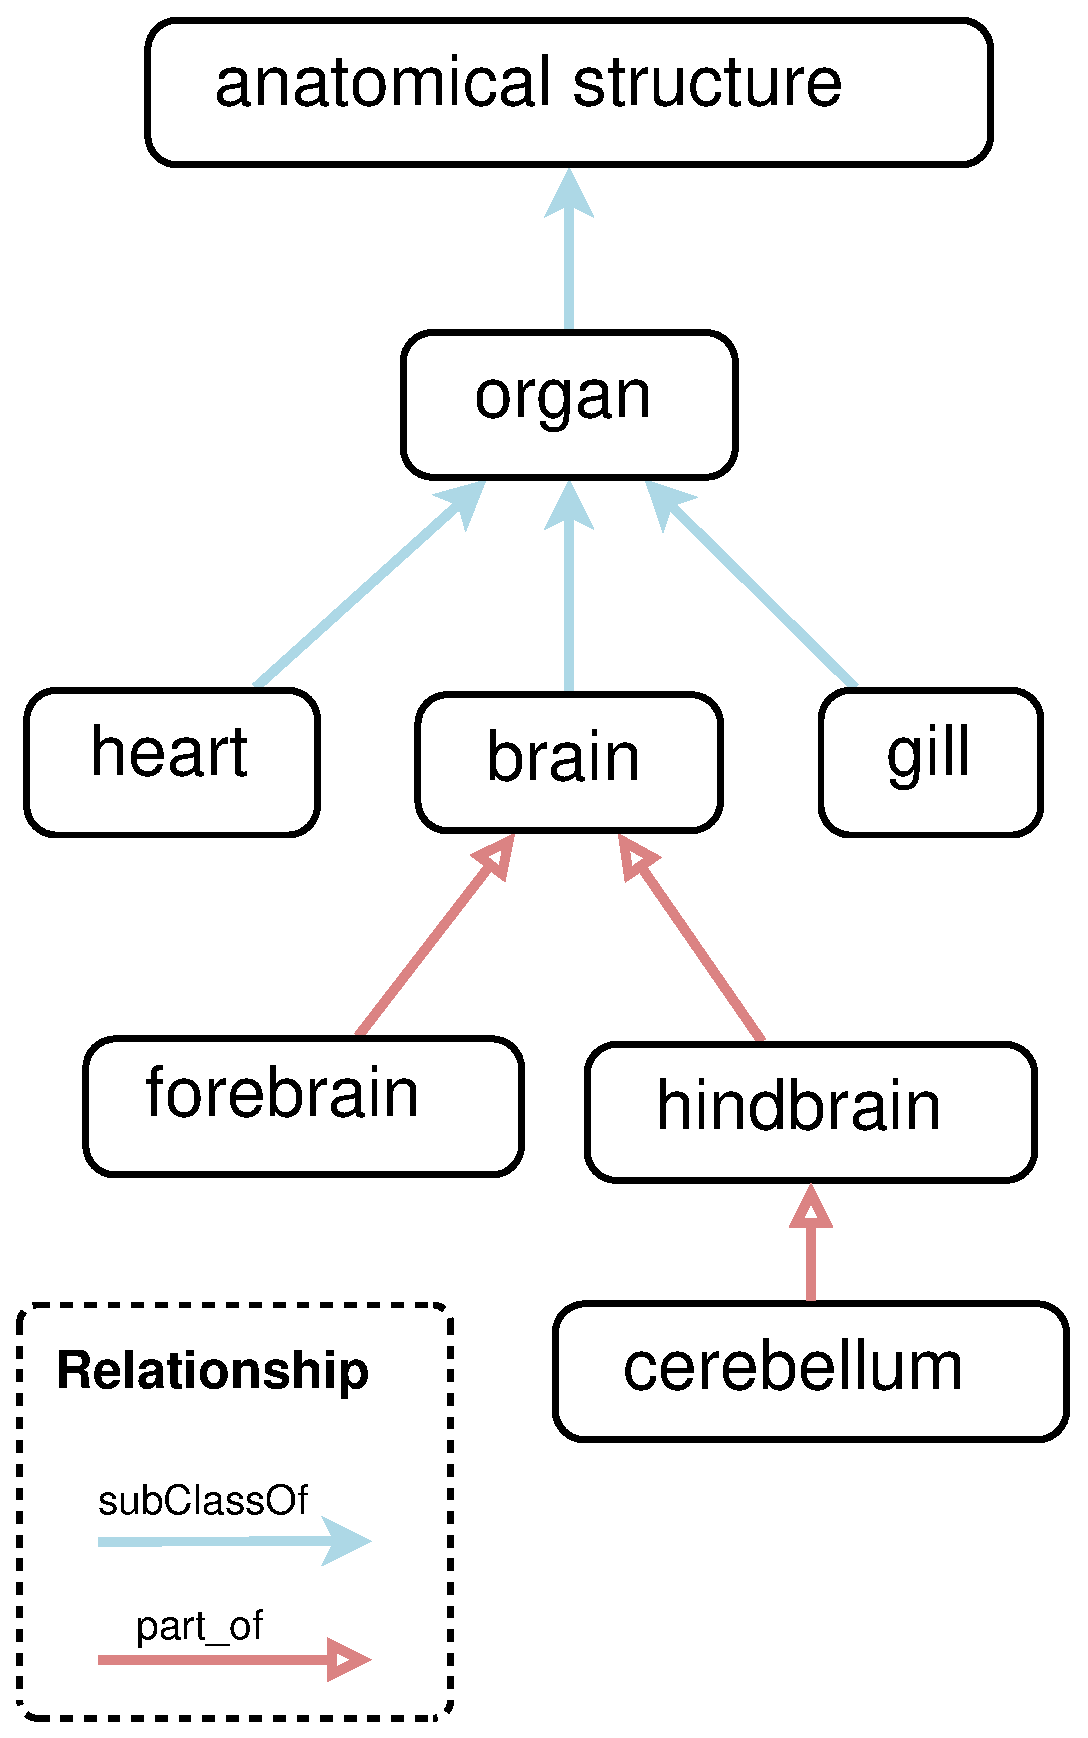
\includegraphics[width=.7\textwidth]{fig/DLG-bio.eps}
%\end{minipage}\hspace{1cm}
%\begin{minipage}[c]{0.5\textwidth}\centering
%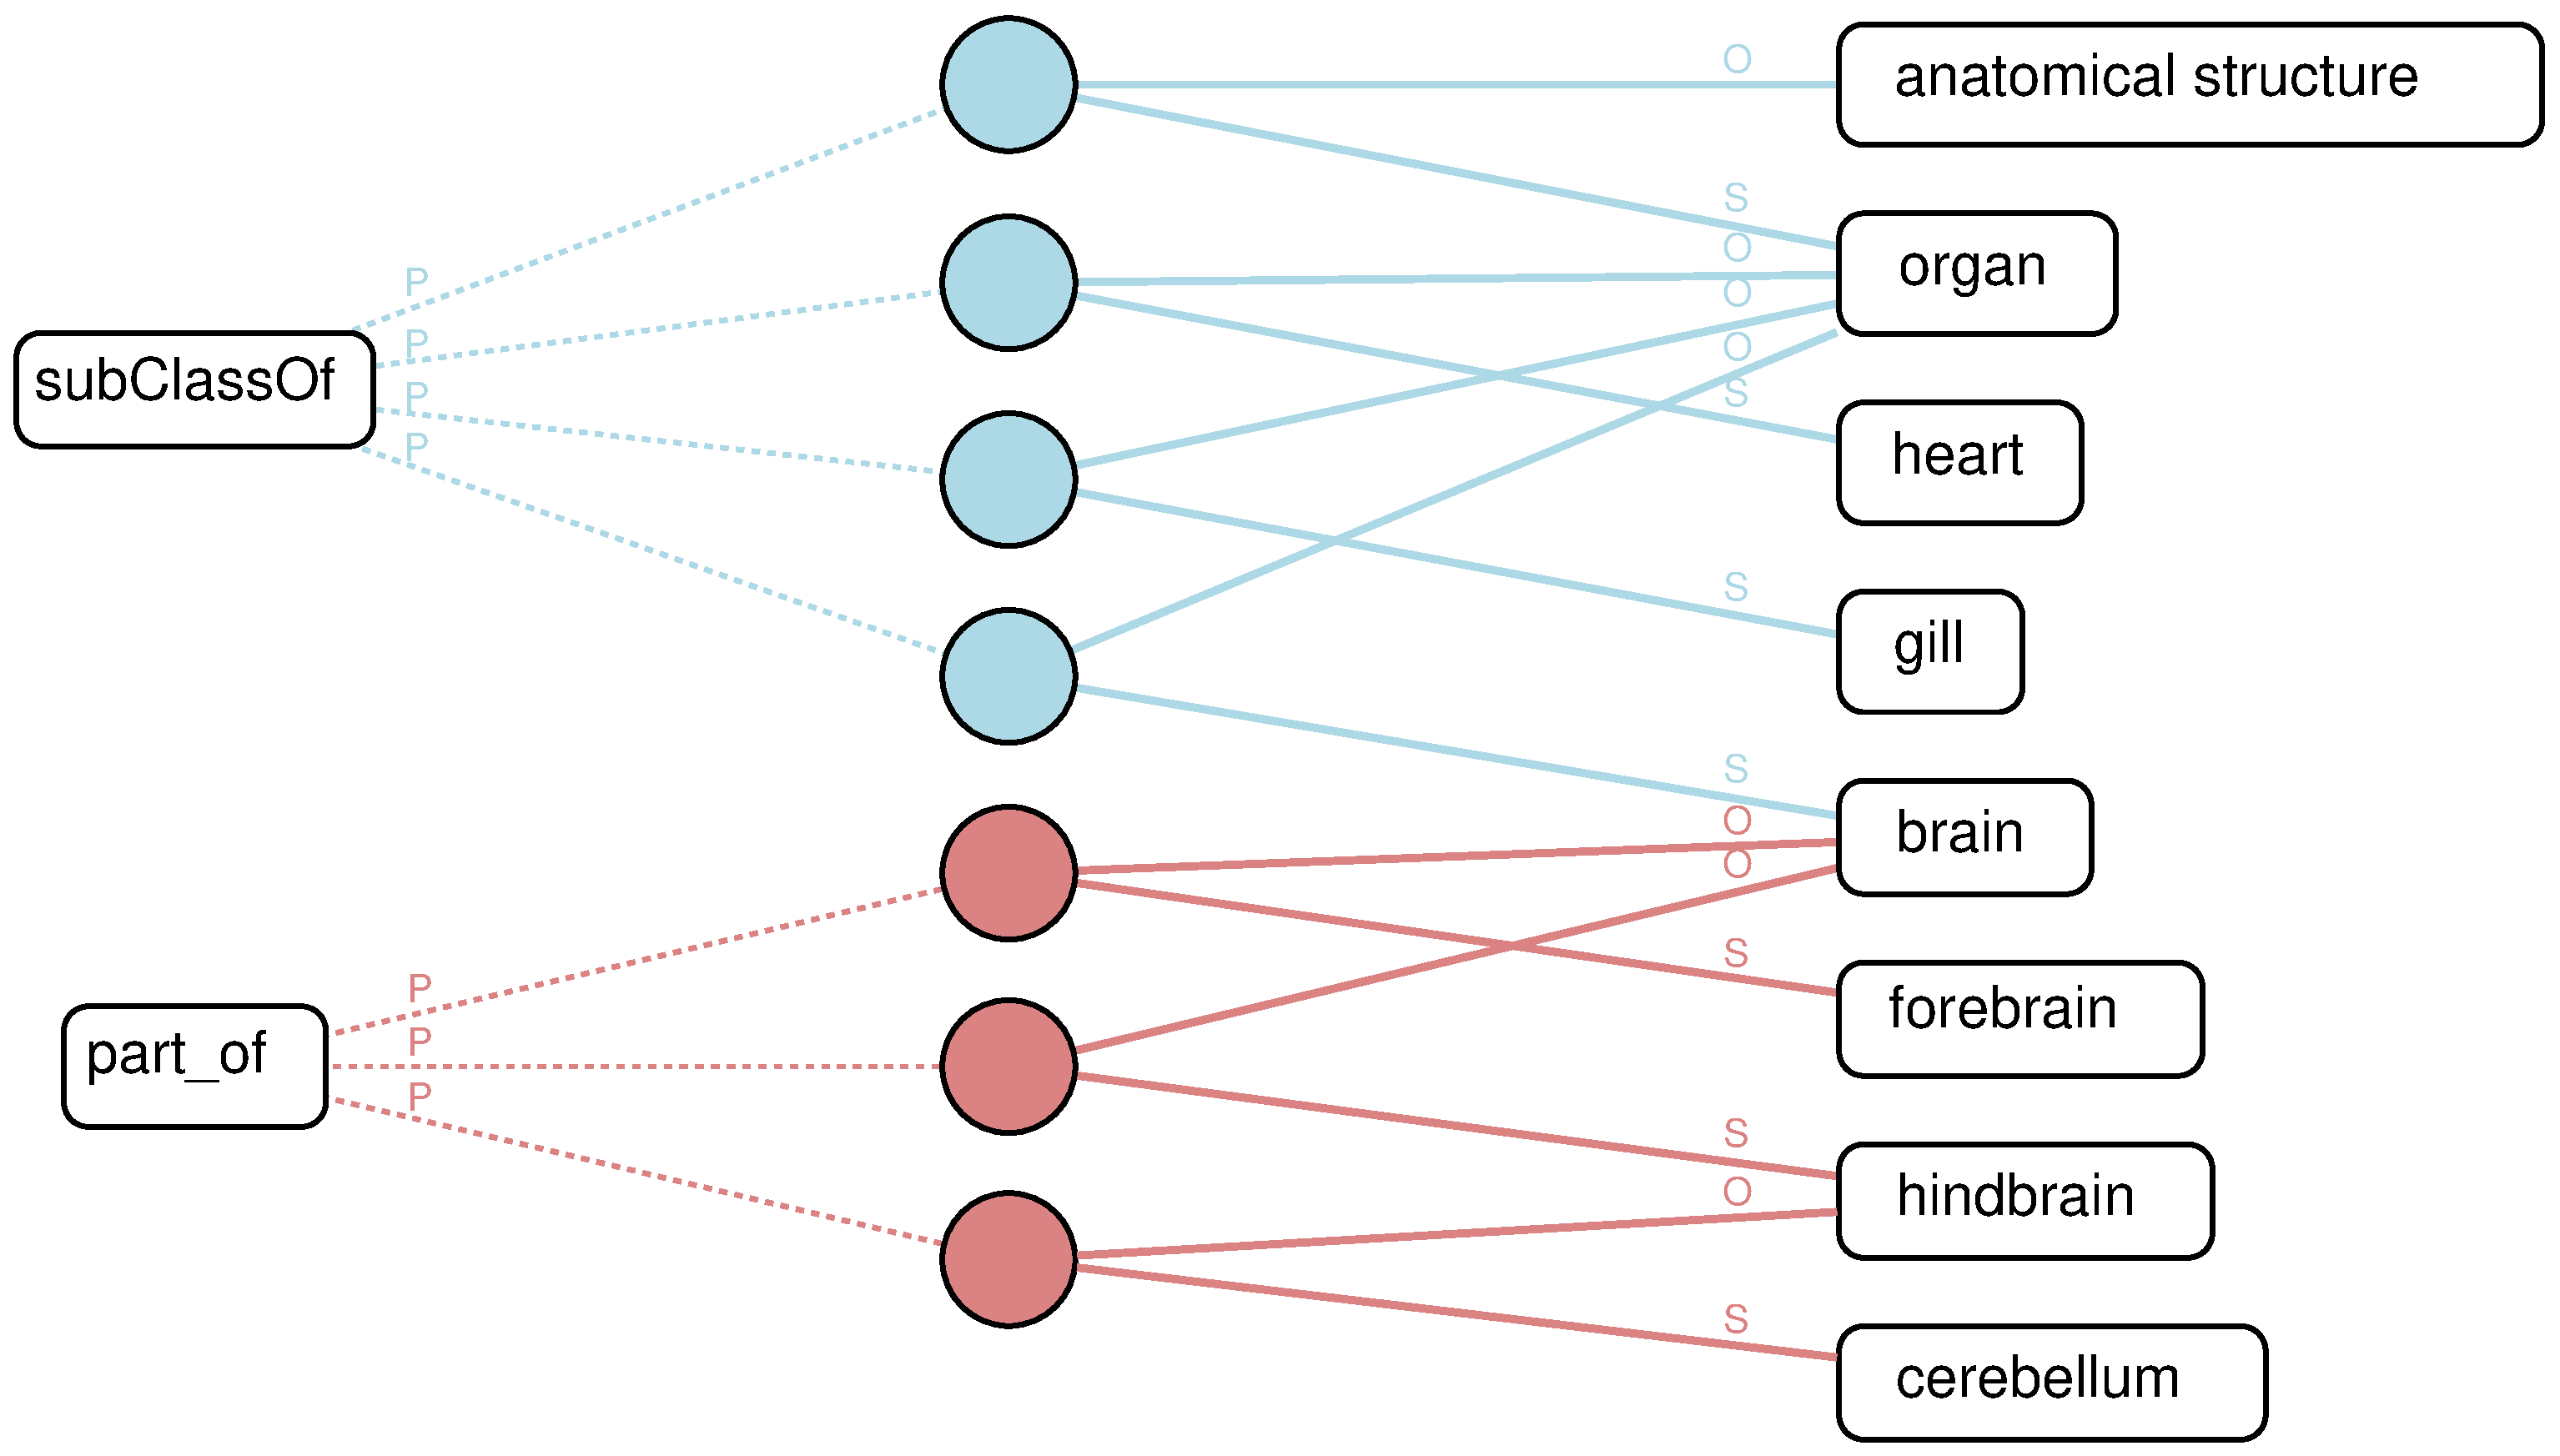
\includegraphics[width=\textwidth]{fig/BG-bio.eps}\\
%\end{minipage}
%\caption{\label{fig:graphcomp-bio} A portion of a zebrafish anatomy ontology represented as a directed labeled graph (left) and a RDF bipartite graph (right)}
%\end{figure*}%
\subsection{Ontology-annotated Data as Bipartite RDF Graphs}
%Various graph representation for relational structure has been proposed in literature to tackle different data mining tasks. In the case of frequent itemset mining, a set of objects with the co-occurrence relationship can be represented as directed or undirected graphs.
%
There already exist methods for transforming data, such as those in relation databases, into RDF~\cite{RDB2RDF}. An ontology-annotation, as we see it, is a binary value representing whether some ontological concept (or class) is associated with some entity.  Often, this means that some concept appears in some document and thus the ontology serves to index the document with related concepts~\cite{RI}.  Thus, we can think of ontology-annotations as a table, with each row representing an entity (e.g., a document), and each column is a class from some ontology.  Cells having a ``1'' denotes that the document \emph{mentions} the term defined by the class.  RDF can be seen as a sparse matrix representation of this data (Table~\ref{tbl:binary-rel}).  This idea can be easily extended to nominal-valued tables as well, or with other relationships besides \emph{mentions} as we illustrate when discussing ontologies as bipartite graphs in the next section.
\begin{table}[ht]
\begin{minipage}[b]{0.38\linewidth}\begin{flushright}
\begin{tabular}{ c | c | c | c |}
\cline{2-4}
	~   & $f_1$	    & $\cdots$  & $f_n$   \\
\cline{2-4}
$r_1:$	&  0  	& $\cdots$   &    1  \\
\cline{2-4}
$\vdots$& $\vdots$  & $\ddots$  & $\vdots$\\
\cline{2-4}
$r_m:$	&  1  	& $\cdots$   &    0  \\
\cline{2-4}
\end{tabular}
\end{flushright}
\end{minipage}
\hfill
\begin{minipage}[b]{0.4\linewidth}
\begin{tabular}{c c c}
\emph{s}&   \emph{p}&  \emph{o}\\
\texttt{<$r_1$}   &    \texttt{mentions}   &  \texttt{$f_n$>}\\
\texttt{<$r_m$}   &    \texttt{mentions}   &  \texttt{$f_1$>}\\
\end{tabular}
\end{minipage}
\begin{minipage}[c]{0.4\linewidth}\centering
\vspace{0.2cm}\hspace{2.8cm}(A)
\end{minipage}
\begin{minipage}[c]{0.4\linewidth}\centering
\vspace{0.2cm}\hspace{3.5cm}(B)
\end{minipage}
\caption{\label{tbl:binary-rel} Ontology-annotated data (A) is a feature matrix attributing classes from ontologies, $f_i$, to entities such as documents, $r_j$, that is easily represented in sparse matrix form using RDF statements (B).}
\end{table}

\subsection{Incorporating Ontologies into Bipartite RDF Graphs}
Given that ontology-annotated data links entities in the data to classes from ontologies, the RDF bipartite graph can also capture relations among classes in the ontology in the same representation. Thus, data mining algorithms will benefit directly from their seamless integration. The following example shows the combination of an ontology graph and a data graph:

\begin{myexp}
\emph{(\textbf{Ontology and data in one bipartite RDF graph})}
Considering just the \emph{rdfs:subClassOf} for illustration (other relationships are treated no differently), Figure~\ref{fig:onto-and-data}(A,B) shows a small hierarchy for concepts \emph{A--E}. Similarly, Figure~\ref{fig:onto-and-data}(C) provides a set of ontology-annotated data. As illustrated earlier, the ontological statements as hyperedges are structurally no different than data-oriented RDF statements. Thus, Figure~\ref{fig:hypergraph-combined} illustrates the combined graph.
\end{myexp}

\begin{figure*}[tbh]
\begin{minipage}[c]{.4\textwidth}\centering
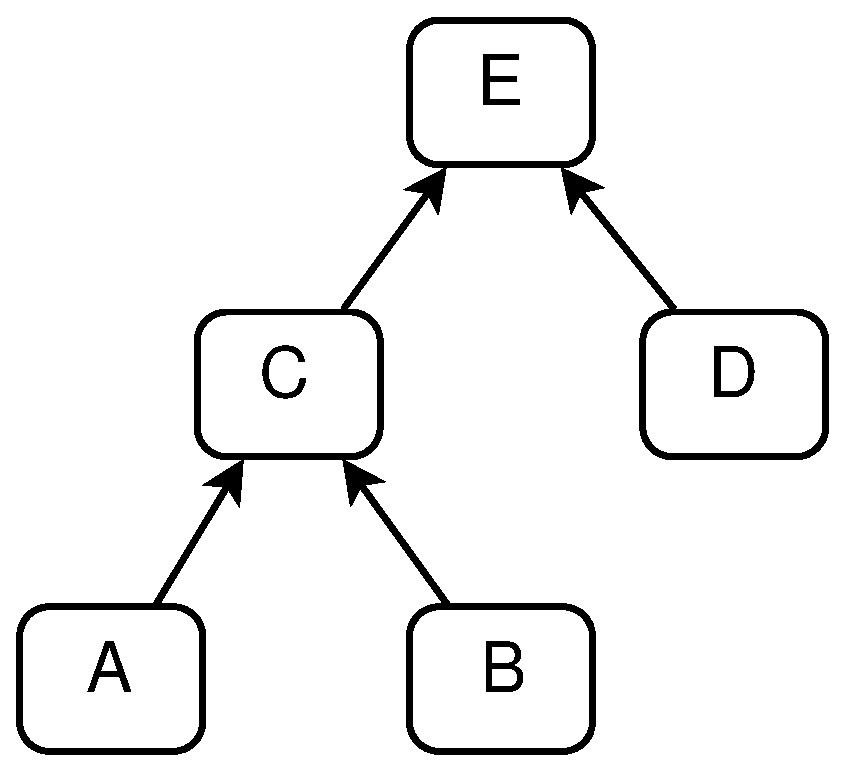
\includegraphics[width=.5\linewidth]{fig/simple-onto.eps}
\end{minipage}
\begin{minipage}[c]{.25\textwidth}\centering
    \begin{tabular}{ c | c | c | c | c | c |}
    \cline{2-6}
    	~ & A & B & C & D & E\\
    \cline{2-6}
    $A:$& 0 & 0 & 1 & 0 & 0 \\
    \cline{2-6}
    $B:$& 0 & 0 & 1 & 0 & 0 \\
    \cline{2-6}
    $C:$& 0 & 0 & 0 & 0 & 1 \\
    \cline{2-6}
    $D:$& 0 & 0 & 0 & 0 & 1 \\
    \cline{2-6}
    $E:$& 0 & 0 & 0 & 0 & 0 \\
    \cline{2-6}
    \end{tabular}
\end{minipage}
\begin{minipage}[c]{.25\textwidth}\centering
    \begin{tabular}{ c | c | c | c | c | c |}
    \cline{2-6}
    	~ & A & B & C & D & E\\
    \cline{2-6}
    $r_1:$& 1 & 1 & 0 & 0 & 0 \\
    \cline{2-6}
    $r_2:$& 1 & 1 & 1 & 0 & 0 \\
    \cline{2-6}
    $r_3:$& 0 & 1 & 1 & 0 & 0 \\
    \cline{2-6}
    $r_3:$& 0 & 0 & 0 & 1 & 0 \\
    \cline{2-6}
    \end{tabular}
\end{minipage}
\begin{minipage}[c]{0.4\linewidth}\centering
(A)
\end{minipage}
\begin{minipage}[c]{0.25\linewidth}\centering
(B)
\end{minipage}
\begin{minipage}[c]{0.25\linewidth}\centering
(C)
\end{minipage}
\caption{\label{fig:onto-and-data} Five concepts (\emph{A--E}) are represented visually as a hierarchy (A) and also as a a hypergraph using the binary feature matrix (B), where a ``1'' denotes \emph{rdfs:subClassOf}, which is similar to the ontology-annotated data (C), where ``1'' denotes \emph{mentions}.}
\end{figure*}

\begin{figure*}[tbh]
\begin{center}
\begin{tabular}{c  c}
\multirow{12}{*}{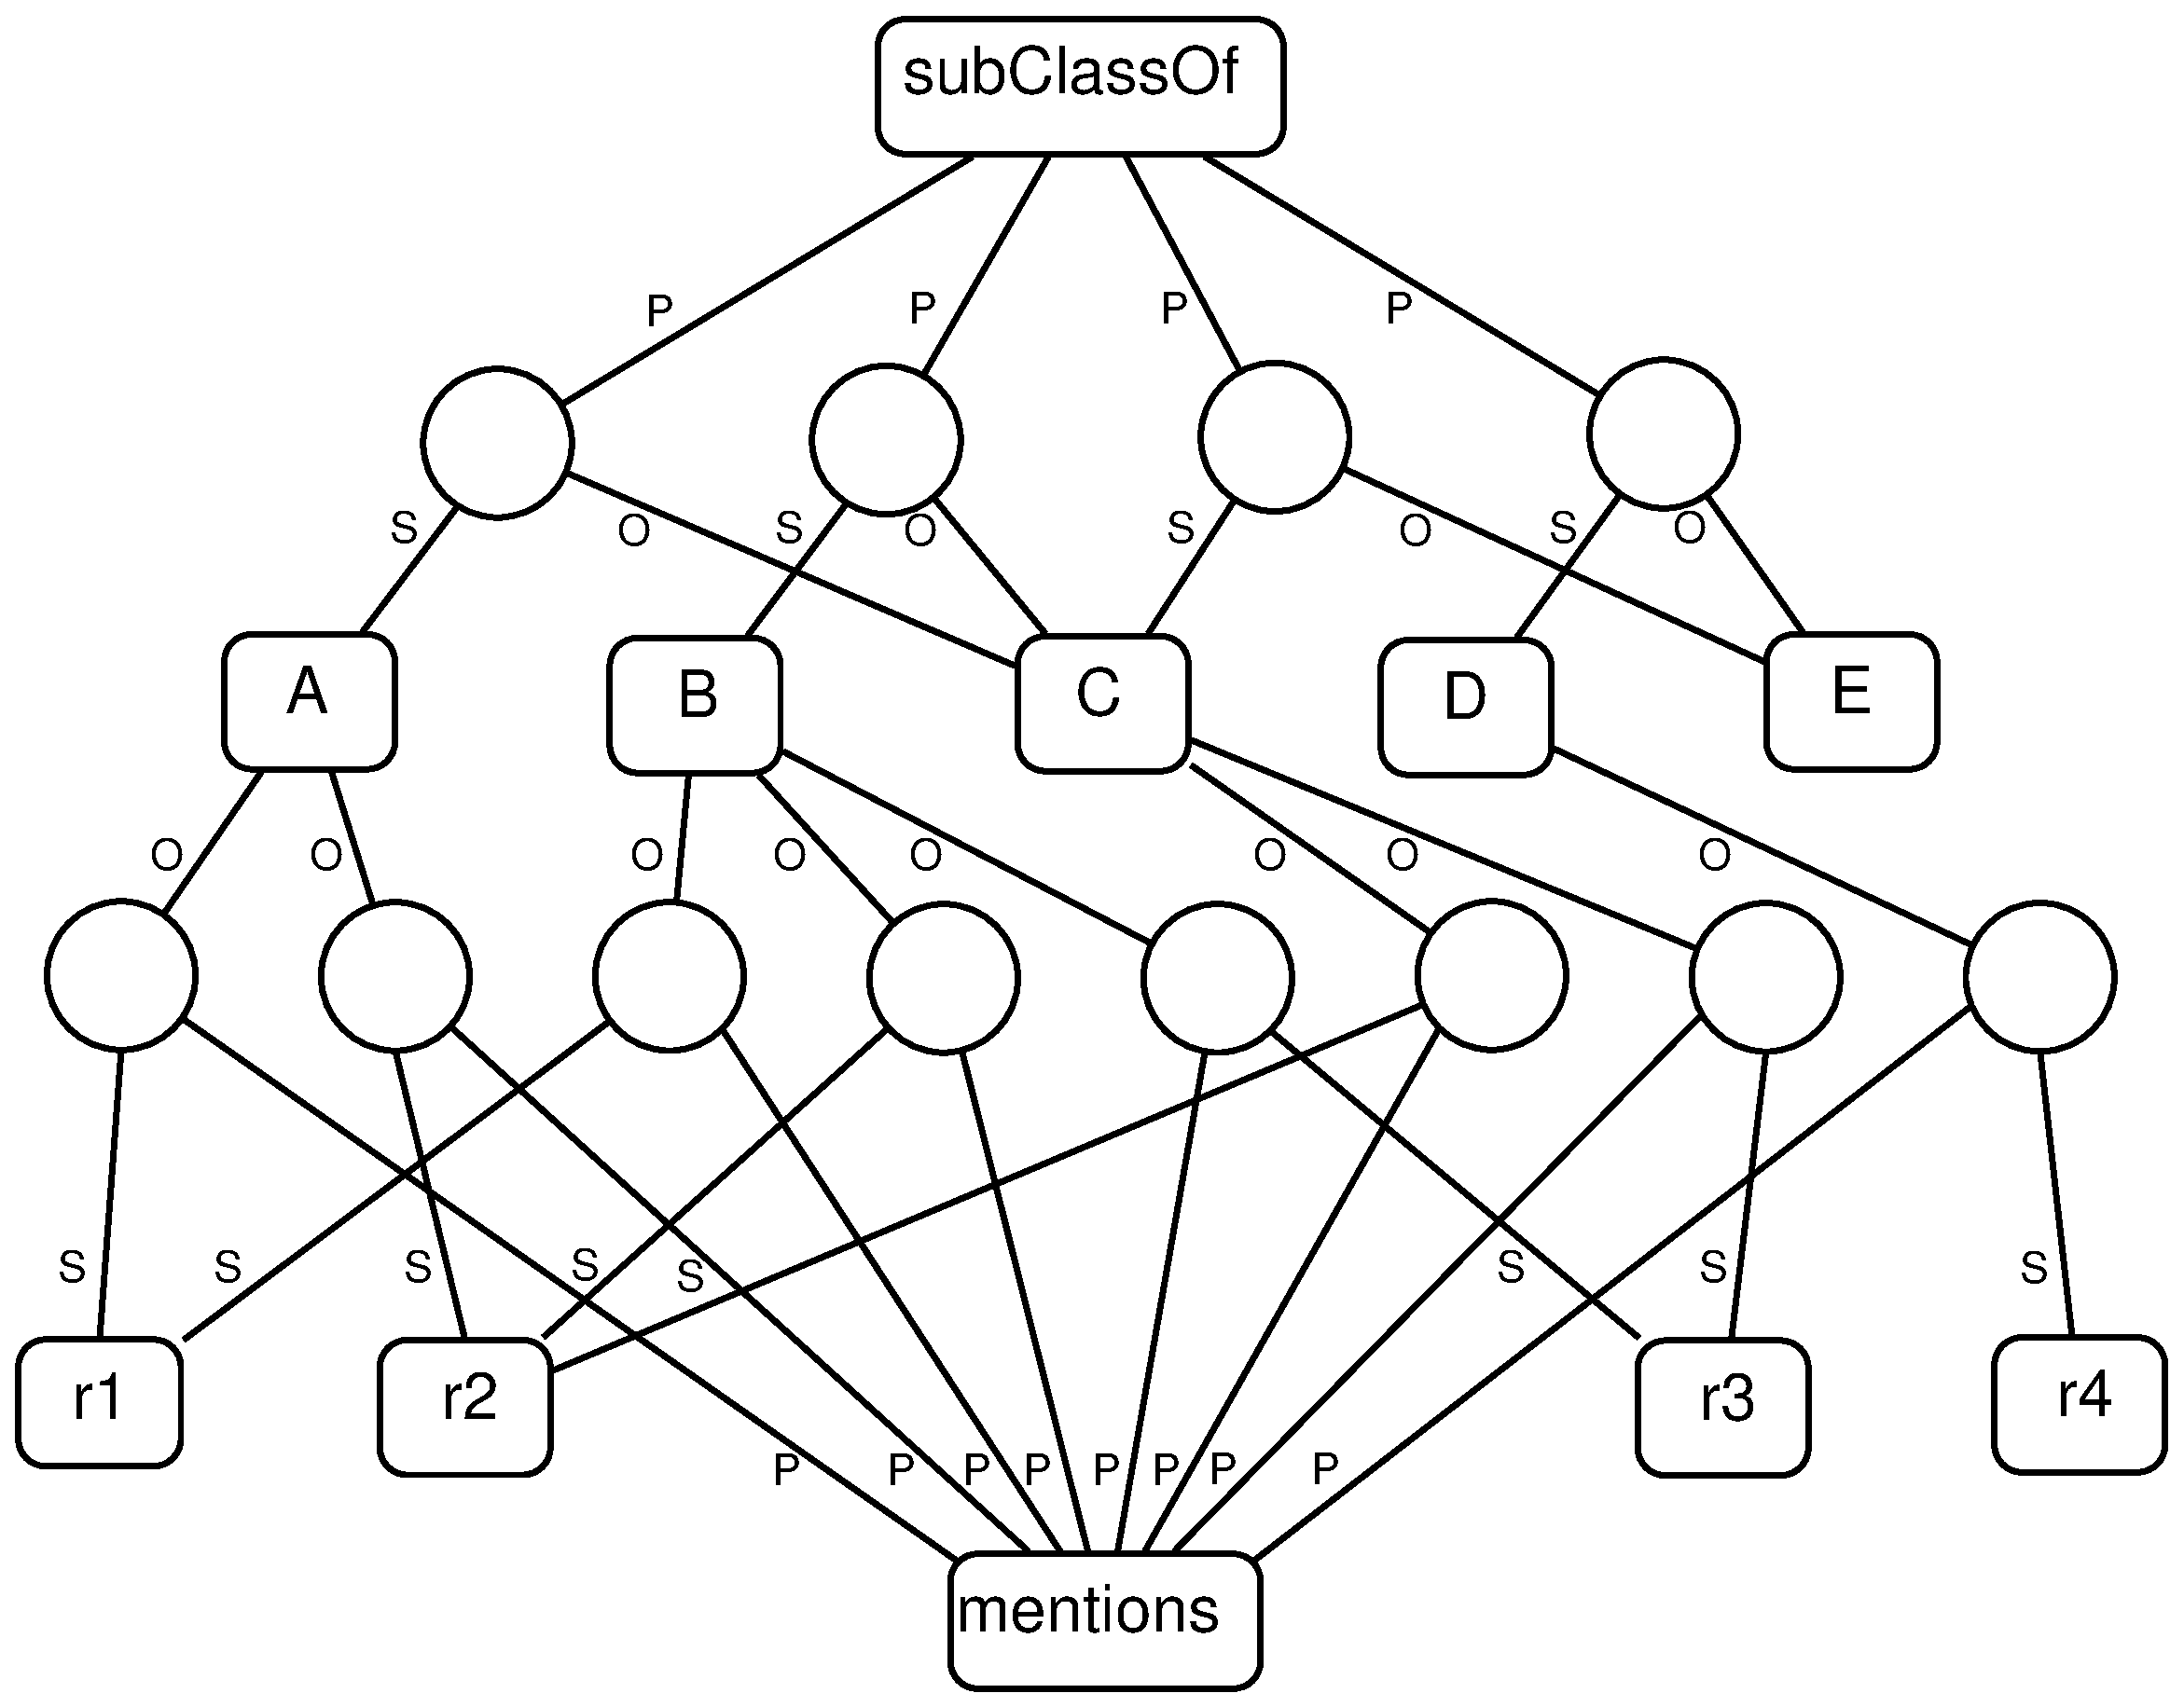
\includegraphics[width=.45\textwidth]{fig/hypergraph_mining.eps}} & \emph{~~~s \hfill p\hfill o~~~}\\
& \texttt{<A>~~<subClassOf>~~<C>}\\
& \texttt{<B>~~<subClassOf>~~<C>}\\
& \texttt{<C>~~<subClassOf>~~<E>}\\
& \texttt{<D>~~<subClassOf>~~<E>}\\
& \\
& \texttt{<r1>\;~~<mentions>\;~~<A>}\\
& \texttt{<r1>\;~~<mentions>\;~~<B>}\\
& \texttt{<r2>\;~~<mentions>\;~~<A>}\\
& \texttt{<r2>\;~~<mentions>\;~~<B>}\\
& \texttt{<r2>\;~~<mentions>\;~~<C>}\\
& \texttt{<r3>\;~~<mentions>\;~~<B>}\\
& \texttt{<r3>\;~~<mentions>\;~~<C>}\\
& \texttt{<r4>\;~~<mentions>\;~~<D>}\\
& \\
& \\
& \\
& \\
(A) & (B)\\
\end{tabular}
\end{center}
\caption{\label{fig:hypergraph-combined} The RDF bipartite graph representation (A) easily combines both the ontology-annotated data with the ontological relationships (B) based on the information described in Figure~\ref{fig:onto-and-data}.}
\end{figure*}

%tripartite view
\begin{figure}[tbh]
\begin{center}
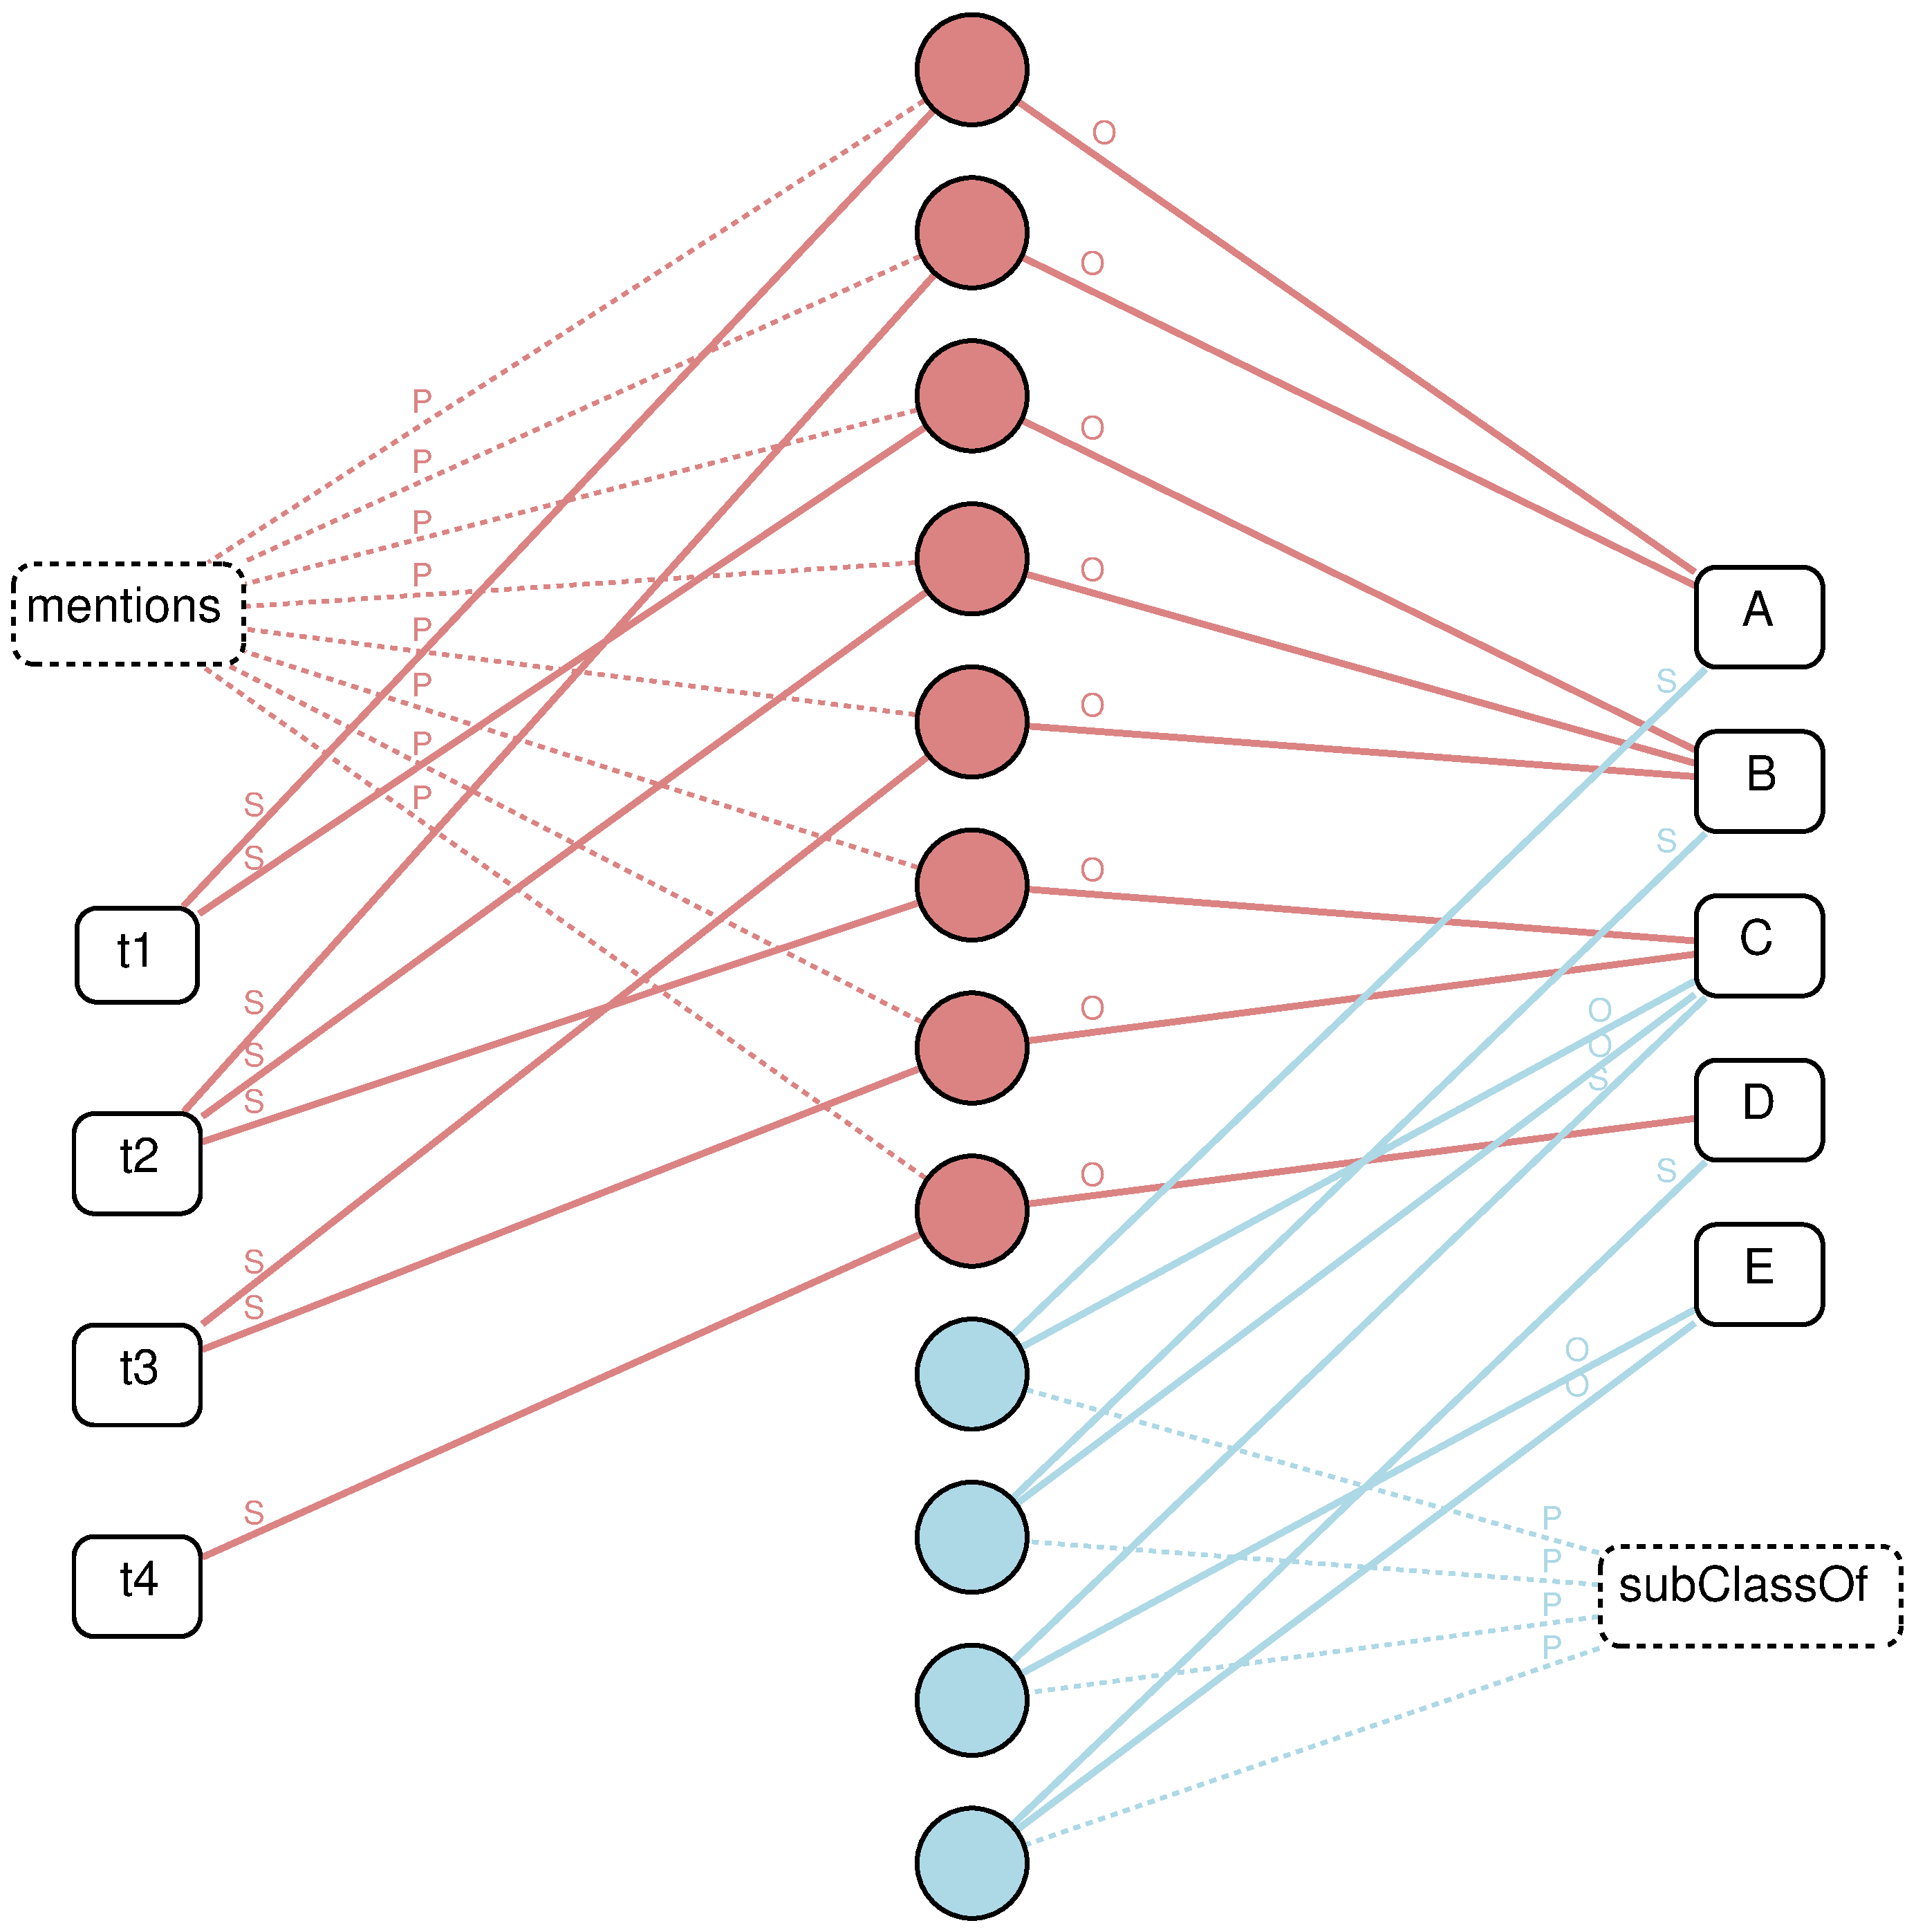
\includegraphics[width=.45\textwidth]{fig/hypergraph_mining-bipartite-weighted.eps}
\end{center}
\caption{\label{fig:bipartitegraph-weighted} By grouping the nodes according to whether they are row elements or column elements in Figure~\ref{fig:onto-and-data} (B), the bipartite graph shown in Figure~\ref{fig:hypergraph-combined} (A) can be further transformed as shown in this figure.}
\end{figure}

Figure~\ref{fig:bipartitegraph-weighted} illustrate another way to view the RDF bipartite graph in Figure~\ref{fig:hypergraph-combined} (A) by visually rearranging nodes. Our proposed semantic association mining algorithm is based on the idea of neighborhood formation using random walk with restart on column nodes (the right most part). Conversely, neighborhood formation on row nodes (the left most part) is able to facilitate row-oriented analysis such as classification and clustering. This shows the flexibility of the RDF bipartite graph in support of different mining tasks. Further discussion can be found in Section~\ref{sec:discussion}.

We also distinguish paths in the RDF bipartite graph by assigning weights to those paths that represent different semantic relationships such as class subsumption, \emph{part\_of}, and other general or domain--specific properties such as \emph{may\_treat}.

%--example of weight assignment
%Figure~\ref{fig:hypergraph_mining-comp} shows an example of RDF bipartite graph representing information on peoples (A--E) where multiple relationships can be identified to link them. E.g., A, B, C and D are linked by the coauthorship relationship, while D and E are linked by the more general collaboration relationship (in fact, coauthorship is defined as a sub-property of collaboration in the ontology). A, B and C are professors, D and E are PhD students, and both professors and PhD students are researchers. In this complex lattice of relationships, we hope to distinguish these relationships by assigning task--specific weights to the related paths (e.g., as conveyed by different colorings in the graph). In order to achieve this, we propose to develop a framework for guiding the (semi-) automatic assignment of weights.
%
%\begin{figure*}[tbh]
%\begin{center}
%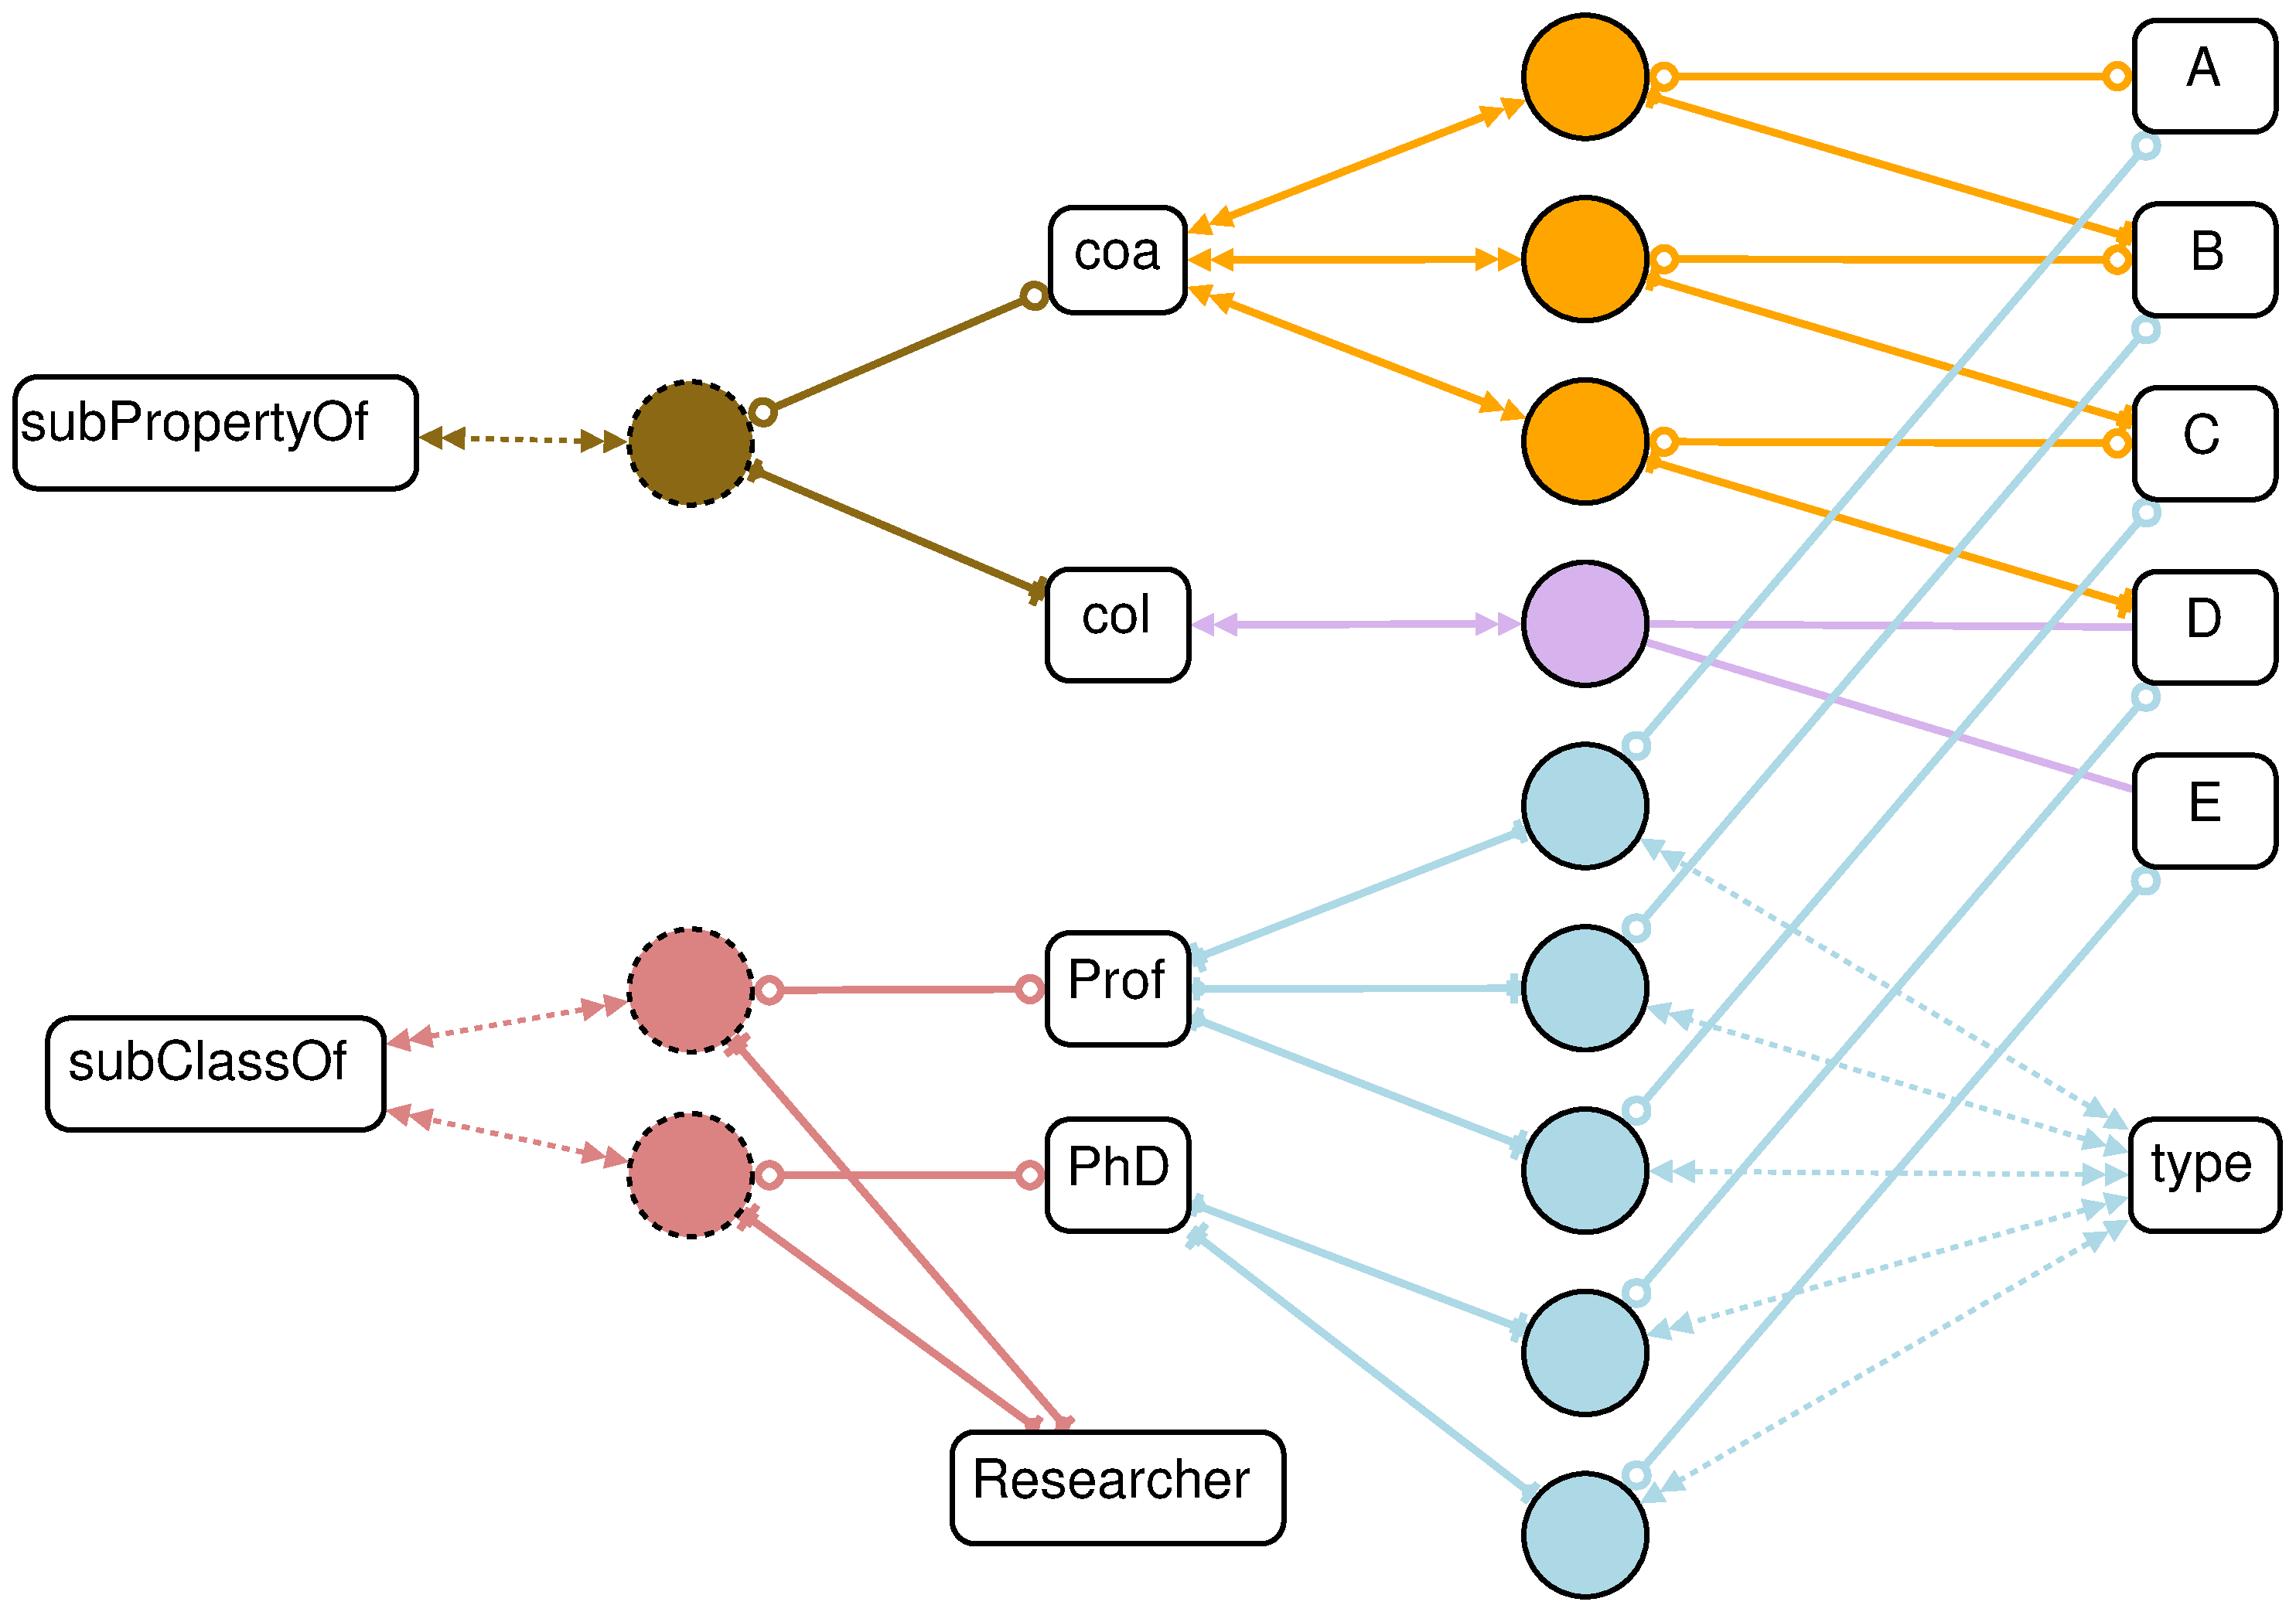
\includegraphics[width=.5\textwidth]{fig/hypergraph_mining-comp.eps}
%\end{center}
%\caption{\label{fig:hypergraph_mining-comp} }
%\end{figure*}

\begin{mydef}
\emph{\textbf{(Data model for the combined RDF bipartite graph)}} The unified RDF bipartite graph of both data and ontology is defined as $G=\langle V_v \cup V_s, E \rangle$, where $V_v$ denotes value nodes corresponding to RDF components (subject, predicate, or object), and $V_s$ denotes statement nodes corresponding to RDF statements. More specifically, statement nodes can be further divided according to whether they are from data or ontology, i.e., $V_s=V_d \cup V_o$; the value nodes can be divided according to whether they represent rows or attributes in the data, i.e. $V_d=V_r \cup V_a$. The graph $G$ can be represented in a biadjacency matrix $\mathbf{M}$, where $\mathbf{M}(i,j)$ is non-zero if there is an edge between $\langle V_{v_i}, V_{s_j} \rangle$. For an unweighted graph, the value can be 0/1, while for a weighted graph, any non-negative value.
\end{mydef}

The biadjacency matrix $\mathbf{M}$ can be split into vertical stripes by statement nodes $V_s$. For example, according to Figure~\ref{fig:hypergraph-combined}(B), the bipartite graph corresponding to lower 8 RDF statements representing the underlying transaction table can be modeled as the matrix $\mathbf{M}_d$ in Equation~\ref{eq:Md} (RDF statement nodes are labeled $s_1\dots s_8$ respectively); and the bipartite graph corresponding to upper 4 statements (labeled $s_9\dots s_{12}$) representing the subsumption hierarchy in the ontology can be modeled as the matrix $\mathbf{M}_o$ in Equation~\ref{eq:Mo}.

To obtain the biadjacency matrix $\mathbf{M}$ of the combined RDF bipartite graph in Figure~\ref{fig:hypergraph-combined}, we can simply concatenate $\mathbf{M}_d$ and $\mathbf{M}_o$ horizontally: $\mathbf{M}=\left[\mathbf{M}_d~\mathbf{M}_o\right]$. In general, If there are $k$ different semantic relationships in the ontology, $\mathbf{M}_o$ can be further divided into more vertical stripes $\mathbf{M}_{o_i}, i=1\dots k$, where $\mathbf{M}_{o_i}$ may represent, for example, the \emph{part\_of} lattice. Each $\mathbf{M}_{o_i}$ is  distinguished from another by the respective weight. In this case, $\mathbf{M}$ is the horizontal concatenation of all the weighted vertical stripes as shown in Equation~\ref{eq:horzcat}. After the concatenation, $\mathbf{M}$ can be represented as the form shown in Equation~\ref{striped_M}.


\begin{equation}\label{eq:Md}
\mathbf{M}_d=\begin{blockarray}{cccccc}
                  ~     &  s_1  &  s_2  &  s_3  & \dots &  s_8  \cr
            \begin{block}{c[ccccc]}
                 r_1    &   1   &   1   &   0   &\multirow{4}{*}{\dots} &   0   \cr
                 r_2    &   0   &   0   &   1   &       &   0   \cr
                 r_3    &   0   &   0   &   0   &       &   0   \cr
                 r_4    &   0   &   0   &   0   &       &   1   \cr
                 %\cline{1-6}
                  A     &   1   &   0   &   1   &\multirow{4}{*}{\dots} &   0   \cr
                  B     &   0   &   1   &   0   &       &   0   \cr
                  C     &   0   &   0   &   0   &       &   0   \cr
                  D     &   0   &   0   &   0   &       &   1   \cr
                  E     &   0   &   0   &   0   &       &   0   \cr
            \end{block}
        \end{blockarray}
\end{equation}

\begin{equation}\label{eq:Mo}
\mathbf{M}_o=\begin{blockarray}{ccccc}
                  ~     &  s_9  & s_{10}& s_{11}& s_{12}\cr
            \begin{block}{c[cccc]}
                 r_1    &   0   &   0   &   0   &   0   \cr
                 r_2    &   0   &   0   &   0   &   0   \cr
                 r_3    &   0   &   0   &   0   &   0   \cr
                 r_4    &   0   &   0   &   0   &   0   \cr
%                 \cline{1-5}
                  A     &   1   &   0   &   0   &   0   \cr
                  B     &   0   &   1   &   0   &   0   \cr
                  C     &   1   &   1   &   1   &   0   \cr
                  D     &   0   &   0   &   0   &   1   \cr
                  E     &   0   &   0   &   1   &   1   \cr
            \end{block}
        \end{blockarray}
\end{equation}

%horizontal concatenation
\begin{equation}\label{eq:horzcat}
\mathbf{M} = \bigg[w_d\mathbf{M}_d ~~ w_{o_1}\mathbf{M}_{o_1} ~~ w_{o_2}\mathbf{M}_{o_2} ~~ \dots\bigg]
\end{equation}

\begin{equation}
\label{striped_M}
\mathbf{M}=\begin{blockarray}{ccccc}
                ~ & ds & os_1 & os_2 & \dots \\
            \begin{block}{c[c|c|c|c]}
                r   &   \mathbf{M}_{dr}  &   \mathbf{0}   &   \mathbf{0}   &   \dots \\
                \cline{2-5}
                a   &   \mathbf{M}_{da}  &   \mathbf{O}_1 &   \mathbf{O}_2 &   \dots \\
            \end{block}
        \end{blockarray}
\end{equation}

The RDF bipartite graph as a unified representation for both ontologies and data serves as the basis for semantic data mining. Given this, the main research challenge is how to develop meaningful graph-based analysis method to utilize the information embedded in this representation. In this work, we focus on tackling one important data mining tasks, namely, {\em association mining}. We will show that, with prior knowledge encoded via ontologies, the unified RDF hypergraphs will enable us to discover hidden association between entities, between entities and ontological concepts, and between ontological concepts.

\subsection{Similarity Ranking by Random Walk with Restart}

Similar to the relevance score~\cite{SunEtal05}, we believe that two items have a strong semantic association if they are related to many similar objects. We apply random walks with restart (RWR) to capture this intuition from the bipartite graph.  We choose the random walk approach to compute the relevance score because it gives nodes that are connected to many other nodes higher ranks, because the random walker has more paths to reach those nodes. The purpose of the periodic restart is to raise the chance that closely related nodes are visited more often than other nodes.

Intuitively, RWR in a bipartite graph works as follows: assume we have a random walker that starts from node $a$. For each step, the walker chooses randomly among the available edges from the current node. After each iteration, with probability $c$, it resets its position back to node $a$. The final steady-state probability that the random walker reaches node $b$ is the similarity score of L with respect to $a$: $s(a, b)$. We denote the similarity score between entities $e_1$ and $e_2$ by $s(e_1, e_2)$, where $s(e_1,e_2) \in [0, 1]$ and $s(e_1, e_2) = 1 \text{ if } e_1 = e_2$ such that an attribute node $a$ in the unified graph $G = G_d \cup G_o$ and $a \in G_d \cap G_o$ we want to compute a similarity score $s(a, b)$ for all nodes $b(\neq a) \in G_d \cap G_o$.

In more detail, given the biadjacency matrix $\mathbf{M}$ in Equation~\ref{eq:horzcat} for the combined RDF bipartite graph $G$, we can construct the adjacency matrix $\mathbf{A}$ of $G$:
\[
\mathbf{A}=\left[
               \begin{array}{cc}
                 \mathbf{0}   & \mathbf{M} \\
                 \mathbf{M}^T & \mathbf{0} \\
               \end{array}
             \right]
\]
The probability of a random walker taking a particular edge $\langle a,b\rangle$ from a node $a$ while traversing the graph is proportional to the edge weight over the total weight of all outgoing edges from $a$, i.e., $P(a,b)=A(a,b)/\Sigma_{i=1}^{m+n}A(a,i)$. Therefore, the Markov transition matrix $P$ of $G$ is constructed as: $P=normc(A)$, where $normc(A)$ normalizes $A$ such that every column sum up to 1.

First, we transform the input attribute node $a$ into a $(k+n) \times 1$ query vector $\mathbf{q}_a$ with 1 in the $a$-th row and 0 otherwise. Second, we need to compute the $(k+n)\times 1$ stead-state probability vector $\mathbf{u}_a$ over all nodes in $G$. Last we extract the probabilities of the row nodes as the similarity score vectors. Note that $\mathbf{u}_a$ can be computed by an iterated method from the following lemma.

\begin{mylem}\label{lem:pi}
Let $c$ be the probability of restarting random-walk from the node $a$. Then the steady-state probability vector $\mathbf{u}_a$ satisfies
\begin{equation}
\mathbf{u}_a=(1-c)P_A\mathbf{u}_a+c\mathbf{q}_a~.
\end{equation}
\end{mylem}

\renewcommand{\algorithmicrequire}{\textbf{Input:}}
\renewcommand{\algorithmicensure}{\textbf{Output:}}
\begin{algorithm}
\caption{Calculate Semantic Association}
\label{alg1}
\begin{algorithmic}
\REQUIRE query attribute $a$, bipartite matrix $M$, restarting probability $c$, tolerant threshold $\epsilon$
\ENSURE $y = x^n$
\STATE $\mathbf{q}_a \Leftarrow \mathbf{0}$
\STATE $\mathbf{q}_a(a)=1$ (set $a$-th element of $\mathbf{q}_a$ to 1)
\WHILE{$|\Delta\mathbf{u}_a| > \epsilon$}
\STATE \[
    \mathbf{u}_a = (1-c)  \left[ \begin{array}{c}
        normc(\mathbf{M})\mathbf{u}_a(k+1:k+n);\\
        normc(\mathbf{M}^T)\mathbf{u}_a(1:k)
    \end{array} \right] + c\mathbf{q}_a
\]
\ENDWHILE
\RETURN $\mathbf{u}_a(1:k)$
\end{algorithmic}
\end{algorithm}

The iterative update of $\mathbf{u}_a$ in the algorithm (inside the while loop) is modified from Lemma~\ref{lem:pi} while avoiding materializing $\mathbf{A}$ and $\mathbf{P}$ for scalability. 